\chapter{Test and Evaluation}
\label{ch:evaluation}
%Aufbau der Messumgebung (1­2 Seiten)
%●
%Server/Betriebssystem etc.
%Datensätze
%Anfragen
%Systeme/Ansätze gegen die Sie sich vergleichen
%Wie messen Sie? Methodik und Maßeinheiten?
%Ist die Messung signifikant?
%Hypothesen/ Was erwarten Sie?
%
%Ergebnisse und Beobachtungen (3 ­4 Seiten)
%●
%Beschreibung  der Ergebnisse
%Diagramme
%Darstellen von Zusammenhängen
%Diskussion und Bewertung (3 ­4 Seiten)
%●
%Wurden Sie überrascht?
%Stimmten Ihre Hypothesen?
%Sind Sie besser, anders als das andere System?
%Wichtigster Erkenntnisgewinn 1
%Wichtigster Erkenntnisgewinn 2
%... .
%Wichtigster Erkenntnisgewinn N
%Anwendbarkeit? Szenario?
%Zusammenfassung (ca. 0,5 Seiten)
%●
%Was haben wir in diesem Kapitel gelernt?
%Wie passt das zur Zielstellung der Arbeit
%Wie passt das zum nächsten Kapitel?
%
%In this section, we will focus on testing and evaluating implemented profiling solution. Testing
%is necessary and extremely important phase in software development lifecycle. For testing
%purposes, we have chosen several approaches:
% manual testing of chosen test scenarios,
% profiling overhead testing with for this purposes designed application,
% profiling overhead and general testing with midPoint
% Automatic testing with unit tests,
%\section{Automated test environment}

The last chapter discussed implementation details for the \textit{"Collector-Platform"} introduced in \autoref{ch:architecture}.
For its realization, Java 8 as programming language head been chosen in combination with the Spring Boot framework which allowed
the rapid implementation of self-containing, distributed applications.

In this section, the focus will be on testing and evaluating the proposed system solution to ensure compliance with the criteria
defined in \autoref{sec:fr} and \autoref{sec:nfr}.

\section{Automated Tests}

A significant approach for testing software products are automated tests that will be executed in the building process.
In Java, unit tests are used for this purpose. The \textit{Collector-Platform} uses Maven as Build-Managemement solution,
that mean the provided test implementations in form of JUnit test classes will be triggered automatically and the sucessfull passing
all existing test cases is a requirement for a successfull building process.

The \textit{"Collector-Platform"}

test
it
coverage



%Prerequisites:
%
%* [java 8](http://www.oracle.com/technetwork/java/javase/downloads/index.html)
%* [maven](https://maven.apache.org/install.html)
%* [docker](https://docs.docker.com/engine/installation/)
%* [docker-compose](https://docs.docker.com/compose/install/
%
%The application was developed and is working with the following software components:
%
%* ubuntu 16.04 LTS
%* oracle java 8
%* maven 3.3.3
%* docker 1.11.2
%* docker-compose 1.7.1

Unit- and Integration tests, IT needs docker infrastructure, usually mocked JMX, REST data,
lack of time, test separation via naming *Test and *IT via Maven Failsafe, check test coverage,
%
%5.4 Automatic Tests
%Another significant approach to testing software products are automatic tests. In java, unit tests
%are used for this purpose. We have implemented automatic tests in our solution using maven
%project management tool and TestNG framework, which provides similar functionality as
%JUnit framework with several new features.
%Scenarios in automatic tests are not that different from scenarios used in automatic
%testing. Main difference is, that in manual tests, living person needed to use applications GUI to
%perform actions defined in test scenarios, while in automatic tests, these test scenarios are
%written as standard java methods with corresponding annotations and no interaction with GUI is
%needed, we simply call specific methods to complete test scenarios (same methods are called in
%manual testing, except they are invoked by user interaction with GUI). For automatic tests, we
%also need to prepare set of test data, for example create necessary profiling objects. We can
%create them programmatically in code of current test code, or prepare them in form of XML and
%parse them during test execution.

\section{Docker environment}

local cluster
Short Docker intro, benefits in microservice environments, describe setup for components (docker-compose.yml),
describe modifications made for Apache Flink and Apache Kafka to enable JMX remote access

\begin{figure}[H]
	\centering
	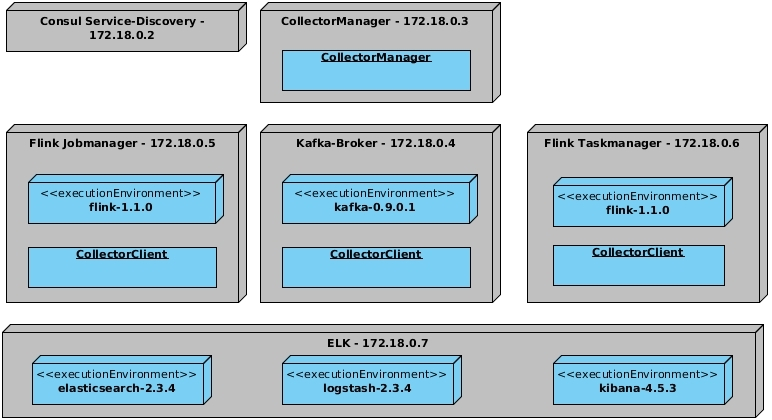
\includegraphics[width=1.0\textwidth]{../uml/deployment-diagram.jpg}
	\caption{Docker Deployment diagram}
	\label{img:deployment-diagram}
\end{figure}

Build images



%\section{Observations}
%
%CollectorDataProcessor: module to analyze the data streams creating derived streams and persist flat
%data -> data transformation, analytics layer
%
%Kibana dashboard, show visualization of CollectorDataProcessor data

\section{Discussion}
%Wurden Sie überrascht? Stimmten Ihre Hypothesen? Sind Sie besser, anders als das andere System?
%Wichtigster Erkenntnisgewinn 1
%Wichtigster Erkenntnisgewinn 2
%Wichtigster Erkenntnisgewinn N
%Anwendbarkeit? Szenario?
\section{Summary}

TODO

%Beschreibung  der Ergebnisse, Diagramme, Darstellen von Zusammenhängen